\documentclass[tikz,border=9pt]{standalone}
\usepackage{amsmath,amssymb}
\usetikzlibrary{arrows.meta,positioning,calc}
\begin{document}
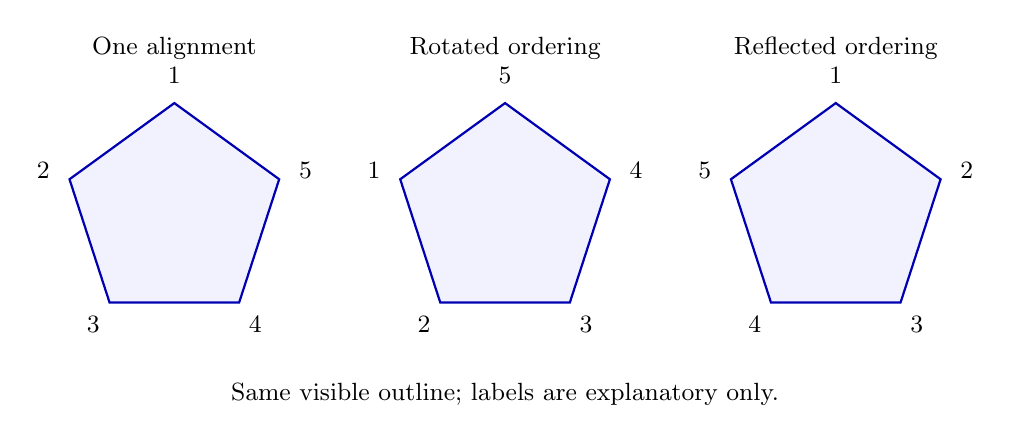
\begin{tikzpicture}[font=\small,arr/.style={-{Stealth},thick},box/.style={draw=blue!55!black,rounded corners,fill=blue!4,align=center,text width=2.9cm,minimum height=1.05cm}]
\draw[thick,blue!70!black,fill=blue!5] (8.572527594031472e-17,1.4)--(-1.3314791228132148,0.43262379212492647)--(-0.8228993532094625,-1.1326237921249263)--(0.8228993532094621,-1.1326237921249265)--(1.331479122813215,0.432623792124926)--cycle;
\node at (0.0,2.1) {One alignment};
\node at (1.071565949253934e-16,1.75) {1};
\node at (-1.6643489035165184,0.540779740156158) {2};
\node at (-1.0286241915118282,-1.4157797401561578) {3};
\node at (1.0286241915118275,-1.415779740156158) {4};
\node at (1.6643489035165189,0.5407797401561575) {5};
\draw[thick,blue!70!black,fill=blue!5] (4.2,1.4)--(2.8685208771867856,0.43262379212492647)--(3.3771006467905376,-1.1326237921249263)--(5.022899353209462,-1.1326237921249265)--(5.531479122813215,0.432623792124926)--cycle;
\node at (4.2,2.1) {Rotated ordering};
\node at (4.2,1.75) {5};
\node at (2.535651096483482,0.540779740156158) {1};
\node at (3.171375808488172,-1.4157797401561578) {2};
\node at (5.228624191511828,-1.415779740156158) {3};
\node at (5.864348903516518,0.5407797401561575) {4};
\draw[thick,blue!70!black,fill=blue!5] (8.4,1.4)--(7.068520877186786,0.43262379212492647)--(7.577100646790538,-1.1326237921249263)--(9.222899353209462,-1.1326237921249265)--(9.731479122813216,0.432623792124926)--cycle;
\node at (8.4,2.1) {Reflected ordering};
\node at (8.4,1.75) {1};
\node at (6.735651096483482,0.540779740156158) {5};
\node at (7.371375808488173,-1.4157797401561578) {4};
\node at (9.428624191511826,-1.415779740156158) {3};
\node at (10.06434890351652,0.5407797401561575) {2};
\node at (4.2,-2.3){Same visible outline; labels are explanatory only.};
\end{tikzpicture}
\end{document}
